The data that an organisation produces can be represented by a Data Virtual Machine (DVM), a conceptual model based on graphs. It provides for quick, ad hoc, on-demand data model development and offers schema flexibility. DVMs provide data sharing, data portability, and a single view of any entity. Data virtualization is an industry concept that is only starting to take off. Data is portrayed in a DVM as nodes and edges in a graph, where the nodes stand in for attributes and entities. By assigning attributes from various data sources to entities or by performing computations, DVMs can be swiftly created. They provide a formalism that makes it possible for non-IT experts to participate in dataframing duties and they enable data exchange and data portability. DVMs can be created quickly and represent the aggregate of calculations carried out on the data infrastructure. The data retrieval operations or computations made on the already-existing data determine the schema of a DVM. They offer an algebraic framework for query evaluation with proven advantages and permit declarative and visual description of dataframes\cite{chatziantoniou}.

\subsection{Data Virtual Machine Structure}

To understand how a DVM works, it can be thought of as an altered ER (Entity-Relationship) model. In an ER model, entities are represented at a higher level, and relationships are depicted between entities using relationship modeling constructs. However, in a DVM, all attributes are \textit{derived} and \textit{multi-valued}, and entities are represented by their \textit{primary attributes}. This means that in a DVM, each node can be considered either as an entity or an attribute, depending on the analysis perspective. A DVM consists of \textit{mappings}, that are represented as edges, between \textit{attribute domains}, that are represented by nodes. Mappings appear as data processes with a 2-dimensional output (the attribute domains)\cite{chatziantoniou}.

For example, in an ER model, attributes are directly associated with entities, and relationships are defined separately. In contrast, in a DVM, attributes are derived through computations and bound to entities via their primary attribute. The primary key of an ER entity now represents the entity itself as a node, associated with other nodes that represent the entity's attributes.

While ER models follow a top-down approach, starting from conceptual design and going towards a logical model, DVMs follow a bottom-up approach, starting from existing data and constructing a conceptual model based on the computations performed on that data\cite{chatziantoniou}.

\textit{Definition 3.1:} \textbf{[Data Virtual Machines]} Assume a collection \(A\) of \(n\) domains \(A_1, A_2, ..., A_n\) called \textit{attributes}. Assume a collection \(S\) of \(m\) multisets \(S_1, S_2, ..., S_m\), where each multiset \(S\) has the form: \(S = \{(u, v): u \in A_i, v \in A_j, i, j \in \{1, 2, ..., n\}\}\), called \textit{data processing tasks}. For each such \(S \in \{S_1, S_2, ..., S_m\}\) we define two key-list structures, \(K^S_i_j\) and \(K^S_j_i\) as:
\begin{itemize}
    \item[] \(K^S_i_j\): for each \(u\) in the set \(\{u: (u, v) \in S\}\) we define the list \(L_u = \{v: (u, v) \in S\}\) and \((u, L_u)\) is appended to \(K^S_i_j\). \(K^S_j_i\) is similarly defined.
\end{itemize}
The DVM is a multi-graph \(G = \{A, S\}\) constructed as:
\begin{itemize}
    \item each attribute becomes a node in \(G\)
    \item for each data processing task \(S\) we draw two edges \(A_i \to A_j\) and \(A_j \to A_i\), labeled with \(K^S_i_j\) and \(K^S_j_i\) respectively.
\end{itemize}
The key-list structure that corresponds to an edge \(e: A_i \to A_j\) is denoted as \(KL(e\), with schema \((A_i, A_j)\)\cite{chatziantoniou}.

\textit{Example 3.1:} Assume two attributes, \texttt{rideID} and \texttt{locationDatetimeID} and the output of te SQL query "\texttt{SELECT rideID, locationDatetimeID FROM taxiRides}" that maps taxi rides and datetime specific locations. The key-list structure of the nodes and edges created by the attributes can be seen in Figure \ref{dvm1}.

\begin{center}
    \begin{figure}[h]
        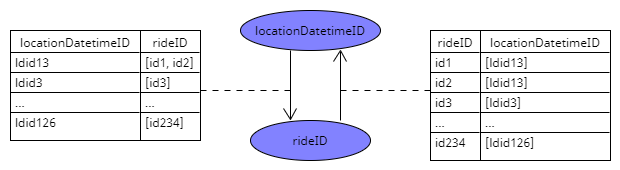
\includegraphics[scale=0.4]{erToDVMExample}
        \caption{ER to DVM representation.}
        \label{dvm1}
    \end{figure}
\end{center}

\subsection{Perfoming queries on DVMs}

To execute our experiments and showcase the usage of a DVM we used the data from the model shown in Figure \ref{dvm2}. They represent taxi rides in New York City in 2022, connected to relevant weather and traffic data. The weather attributes shown in the model, \texttt{snowProb, humidity, rainProb, temperature, datetime, location},  were collected by the \href{https://www.visualcrossing.com/}{Visual Crossing} service for the year 2022 in the city of New York. The traffic data, \texttt{meanSpeed, meanCongestion, datetime, location}, were gathered from \href{https://opendata.cityofnewyork.us/}{NYC Open Data}, which publishes free, public, up-to-date datasets from the city of New York. The attributes concerning the taxi rides, \texttt{DOLocation, PULocation, passengerFare, driverTip, requestDatetime, triverPay, tripTime, tripMiles, airportFee}, were taken from a dataset published by the \href{https://www.nyc.gov/site/tlc/about/tlc-trip-record-data.page}{NYC Gov} website. The datasets from NYC Open Data and NYC Gov used an area code to describe location. In order to match datetime and location data with the other data sources, the area codes were mapped using a complementary dataset to NYC districts and specific areas. After the mapping, the \texttt{requestDatetime} and \texttt{PULocation} from the taxi data attributes were concatenated and hashed using the MD5 hashing method to produce the \texttt{locationDatetimeID} attribute The same was done to the \texttt{location} and \texttt{datetime} attributes for weather and traffic. This action produced a primary attribute that connected all different data sources. Finally, the \texttt{passengerReview} attribute and the \texttt{driverID, gender, vehicleModel, driverUID} were added from two \href{https://www.kaggle.com/}{Kaggle} dataseta that contained customer reviews and driver data for Uber rides. Because most of our data was in CSV form we did some refactoring to test our assumptions under different kinds of data sources. Firstly, the dataset containing the taxi rides was turned into a PostreSQL relational database. The database contained four tables \texttt{trip\_details, trip\_time, trip\_speed} and \texttt{trip\_location}. The attributes were split between those tables and had as primary key a unique integer number called \texttt{intID} and as secondary key the \texttt{locationDatetimeID}. A schema representation can be seen in Figure \ref{schema}. For the rest of the data, the passenger review data were turned in XML format, the weather data in Excel and the traffic and Uber drivers data were kept in a CSV format.

\begin{center}
    \begin{figure}[h]
        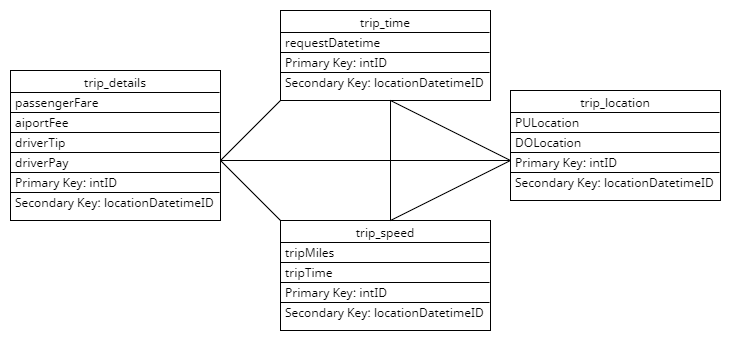
\includegraphics[scale=0.3]{figures/schema.png}
        \caption{Schema representation of taxi rides relations database.}
        \label{schema}
    \end{figure}
\end{center}

It is worth noting that the datasets contained many more attributes than the ones shown in Figure \ref{dvm2}. The purpose of the graphical representation is to highlight the main fields used in our analysis and create a comprehensive conceptual image. Also, the names of the attributes shown in Figure \ref{dvm2} do not match accurately to the ones in the datasets. This was done in order to have more easily understandable naming conventions across the different data sources in the conceptual image that we created.

\begin{center}
    \begin{figure}[h]
        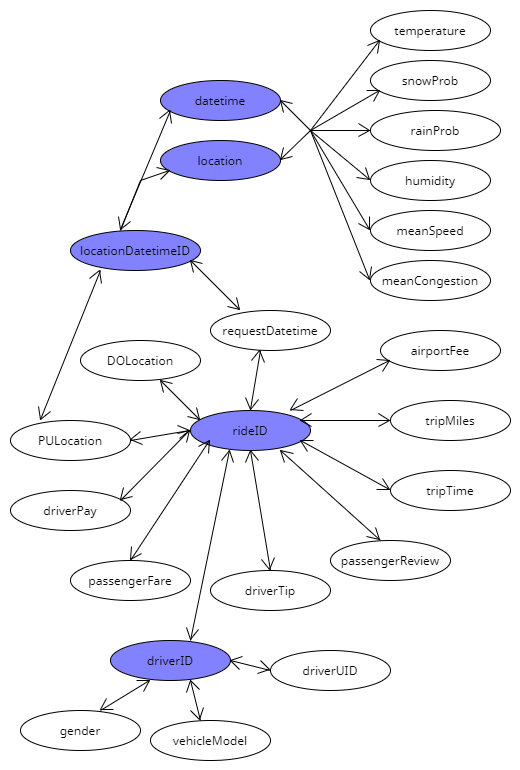
\includegraphics[scale=0.3]{generalDVMView}
        \caption{DVM view of our data.}
        \label{dvm2}
    \end{figure}
\end{center}

With that in mind, a dataframe query over the data is defined by Chatziantoniou et. al. (2022)\cite{chatziantoniou} in Definition 3.2.

\textit{Definition 3.2:} \textbf{[Dataframe Queries]} Given a DVM \(G = \{A, S\}\), a dataframe query is a tree structure \(Q\), defined as:

\begin{itemize}
    \item each node \(N\) of \(Q\) has a \textit{name} and a \textit{label}: the name is unique within \(Q\) and the label is an attribute of \(G\); these are denoted as \(N.name\) and \(N.label\) respectively
    \item for each edge \(N \to N^'\) in \(Q\), there exists an edge: \(label(N) \to label(N^')\) in \(D\)
    \item each edge \(e\) of \(Q\) is annotated with a list of transformations, called the \textit{transformations string}, denoted as \(e.transformations\)
    \item each node \(N\) of \(Q\) is annotated with the \textit{selection condition}, which is either the special value \texttt{'True'} of a python like logical expression, where \(N\) and any of \(N\)'s children may appear as identifiers within this expression; the selection condition of \(N\) is denoted as \(N.selection\)
    \item each node, except the root, has an \textit{output label}, which has the value \texttt{'true'} or \texttt{'false'}; if the output label of a node is \texttt{'true'}, then all nodes in the path from the root to that node, except the root, must have a \texttt{'true'} output label; the output label of the node is denoted as \(N.output\)
\end{itemize}

An example of a dataframe query over the data described above can be seen in Figure \ref{query1}. The root could also be any other attribute of our data, such as \texttt{meanSpeed, passengerReview} etc. 

\begin{center}
    \begin{figure}[h]
        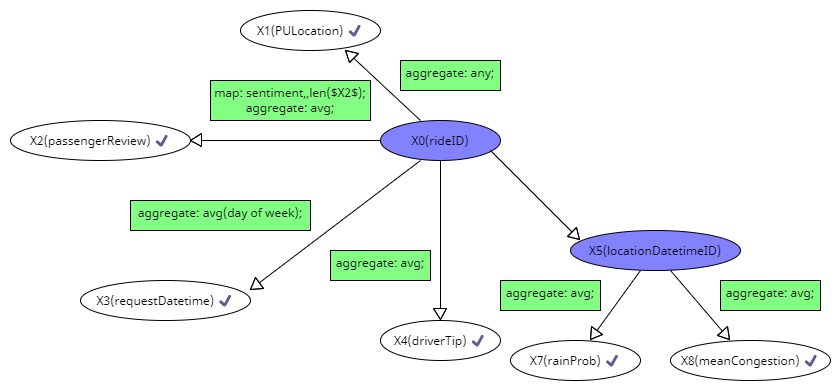
\includegraphics[scale=0.3]{query1}
        \caption{Query tree representation.}
        \label{query1}
    \end{figure}
\end{center}

\subsection{Dataframe query operators}

To evaluate a dataframe query such as the one shown in Figure \ref{query1}, some algebraic operators need to be defined. These operators take as input one or more edges is a key-list structure and produce as output a single edge. We can see some of these operators in Definitions 3.3, 3.4, 3.5, 3.6 and 3.7\cite{chatziantoniou}. An in-depth look and analysis of these operators can be seen in the work by Chatzianotniou et. al. (2022)\cite{chatziantoniou}

\textit{Definition 3.3:} \textbf{[Aggregation]} We define an operator called \textit{aggregation}, which gets a key-list structure \(K\) and an aggregate function \(f\) and returns a new key-list structure \(K^'\) constructed as follows: \(\forall k \in keys(K)\), it adds pair \((k, L_k^')\) to \(K^'\), where \(L_k^{'} = [f(L_k)]\), i.e. a list with a single element, the result of the reduced list \(L_k\) according to \(f\). We denote this operator as \(Aggr(K, f)\)\cite{chatziantoniou}. An example of an aggregated function can be the min, max, average, sum or count functions written in any programming language.

\textit{Definition 3.4:} \textbf{[Filtering]} We define an operator called \textit{filtering}, which gets a key-list structure \(K\) and a condition \(\theta\) defined on a single element of a list (a string) and returns a new key-list structure \(K^'\) constructed as follows: \(\forall k \in keys(K)\), it adds to \(K^'\) a pair \((k, L_k^{'})\), where \(L_k^'\) contains all \(x \in L_k\) such that \(\theta(x)\) is true. We denote this operator as \(Filter(K, \theta)\)\cite{chatziantoniou}.

\textit{Definition 3.5:} \textbf{[Mapping]} we define an operator, called \textit{mapping}, which gets as key-list structure \(K\) and a function \(f\) with a signature \texttt{string f(x:string)} and returns a new key-list structure \(K^'\) constructed as follows: \(\forall k \in keys(K)\), it adds to \(K^'\) a pair \((k, L_k^{'})\), where \(L_k^{'} = [f(x): x \in L_k]\), i.e. each element \(x\) in \(L_k\) is replaced by \(f(x)\). We denote this operator as \(Map(K, f)\)\cite{chatziantoniou}. An example of a mapping can be the transformation of customer reviews to sentiment scores using sentiment analysis.

\textit{Definition 3.6:} \textbf{[RollupJoin]} We define an operator, called \textit{RollupJoin}, which gets two key-list structures \(K_1\) and \(K_2\) and returns a new key-list structure \(K\) constructed as follows: \(\forall k \in keys(K_1)\), it adds to \(K\) a pair \((k, L_k)\), where \(L_k = \oplus_{x \in list(k, K_1)}list(x, K_2)\), \(\oplus\) stands for list concatenation. We denote this operator as \(rollUpJoin(K_1, K_2)\)\cite{chatziantoniou}.

\textit{Definition 3.7:} \textbf{[ThetaCombine]} Given:
    \begin{itemize}
        \item a list \(O\) of key-list structures \(K_1, K_2, ..., K_n\), called the \textit{output} list (can be empty)
        \item a list \(S\) of key-list structures \(K_1^{'}, K_2^{'}, ..., K_m^{'}\), called the \textit{selection} list (can be empty)
        \item a boolean expression \(\theta(k, l_1, l_2, ..., l_m)\) involving \(k\) (an atomic value), \(l_1, l_2, ..., l_m\) (lists of values), called the \textit{selection condition}
    \end{itemize}
we define an operator called \textit{ThetaCombine}, denoted as \(thetaCombine(O; S; \theta)\), which returns a key-list structure \(K\) constructed as follows:
\begin{itemize}
\item[] \(\forall k \in keys(K_1)\cap...\cap keys(K_n)\cap keys(K_1^{'}) \cap...\cap keys(K_m^{'})\):

   \quad if \((\theta (k, list(k, K_1^{'}), ..., list(k, K_m^{'})))\) is true:
        
        \quad \quad add a pair \((k, L_k)\) to \(K\), where:
            
            \quad \quad \quad if \(O\) is empty then \(L_k = []\) (the empty list)
            
            \quad \quad \quad else \(L_k = \oplus_{i = 1, 2, ..., n}list(k, K_i)\)\cite{chatziantoniou}
\end{itemize}

\subsection{Performing DVM queries using DataMingler}

\subsubsection{DataMingler}

DataMingler is a prototype GUI tool to (a) define and manage DVMs, (b) express dataframe queries in a visual and intuitive way, and (c) materialize the DVM (or parts of it) in other logical models – currently only JSON is supported. Data Canvas is the module that enables the creation and manipulation of a DVM by mapping data and processes onto the graph and extending it with new nodes and edges. The data source types that DataMingler currently handles are: relational databases, csv files, excel and stand-alone programs (Java and Python). A DVM is kept in a Neo4j graph database. Dataframe queries can be formulated either textually or visually, using the Query Builder module. In both cases, queries are represented in an XML-based intermediate representation and then parsed and transformed to a key-listalgebraic expression, which is given to the optimizer and an execution plan is generated. Redis is used as the key-value engine for manipulating key-list structures. The JSON Exports module can be used to instantiate model specific databases (currently, JSON is supported). The user selects a node and a breadth-first-search tree rooted on this node is defined. Then the system generates collection of JSON documents corresponding to this tree\cite{chatziantoniou}.

\subsubsection{Query performance}

To test the performance of the DataMingler tool we created a set of queries whose execution time was both tested using the tool and traditional data analysis techniques. In particular, we created Jupyter Notebooks that performed the queries using the Python Pandas library and compared the execution time against the DataMingler tool. It is worth noting that apart from performance, the DataMingler tool should be looked at under the scope of ease-of-use and the need for less technical skills to perform queries on multiple data sources. The creation of these notebooks and management of such different data sources is a highly technical and time consuming task. Having a tool that can accelerate the process without any technical knowledge offers many benefits and can save valuable time and resources.

\textbf{Query 1} For each day of the week we want to have the average, minimum, maximum, count and sum of the \texttt{airportFee, driverPay, tripTime, tripMiles, passengerFare} and \texttt{driverTip}. Also we would like to map the \texttt{passengerReviews} to a sentiment score using a sentiment analysis tool to also show the average, minimum, maximum, count and sum of the reviews for each day of the week. A graphical representation of this dataframe query on DVM can be seen in Figure \ref{queryExp1}.

\begin{center}
    \begin{figure}[h]
        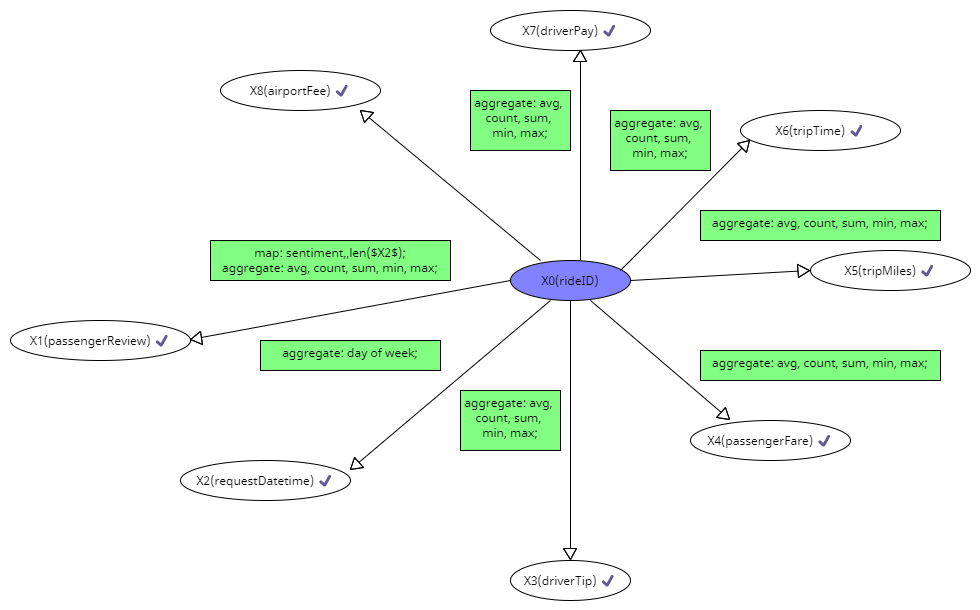
\includegraphics[scale=0.25]{queryExp1}
        \caption{First query of experiment.}
        \label{queryExp1}
    \end{figure}
\end{center}

\textbf{Query 2} For each driver, represented by a unique \texttt{driverUID}, show their \texttt{vehicleModel} and \texttt{gender} along with the average, minimum, maximum, count and sum of their trips \texttt{driverPay, airportFee, passengerReview, driverTip, passengerFare, tripMiles} 
 and \texttt{tripTime}. For the \texttt{passengerReview} the attribute is first going to be mapped using a sentiment analysis tool and then aggregated. A graphical representation of this query on DVM can be seen in Figure \ref{queryExp2}.

\begin{center}
    \begin{figure}[h]
        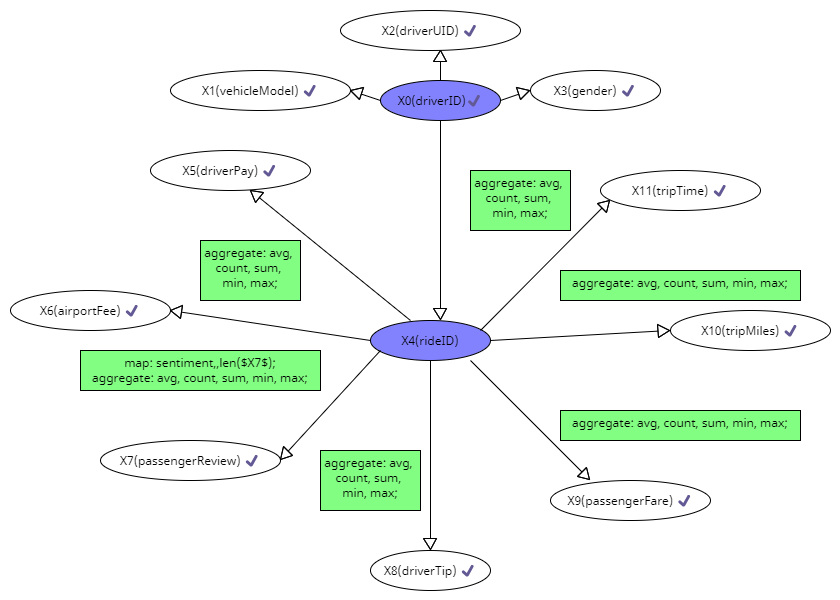
\includegraphics[scale=0.25]{queryExp2}
        \caption{Second query of experiment.}
        \label{queryExp2}
    \end{figure}
\end{center}

\textbf{Query 3} For every location and datetime that taxi trips occurred, represented by \texttt{locationDatetimeID}, show the minimum, maximum, count and sum of the \texttt{airportFee, passengerReview, driverTip, driverPay, passengerFare, tripMiles} and \texttt{tripTime} along with their \texttt{meanCongestion} and \texttt{meanSpeed}. For the \texttt{passengerReview} the attribute is first going to be mapped using a sentiment analysis tool and then aggregated. A graphical representation of this query on DVM can be seen in Figure \ref{queryExp3}.

\begin{center}
    \begin{figure}[h]
        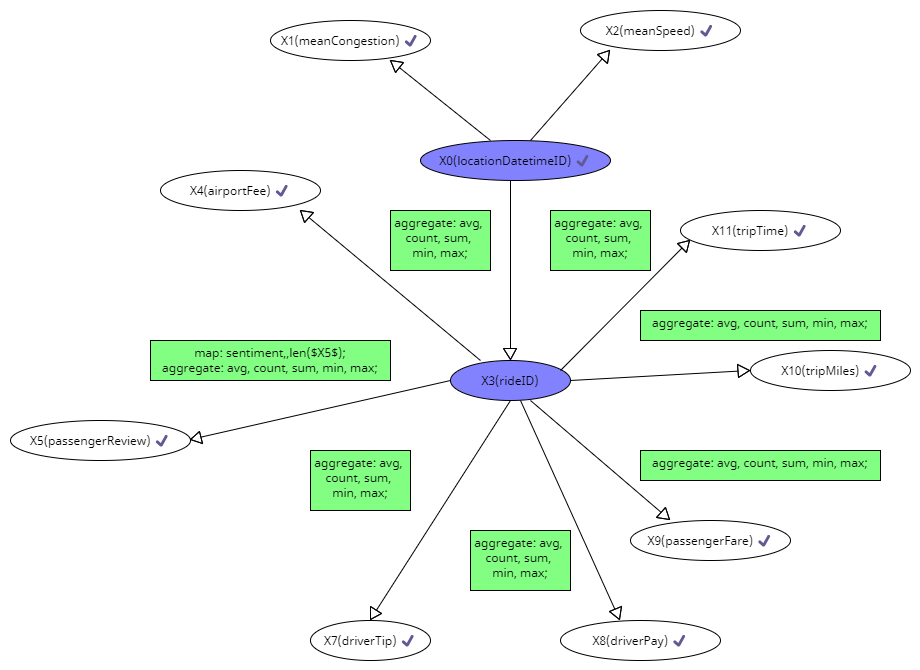
\includegraphics[scale=0.25]{queryExp3}
        \caption{Third query of experiment.}
        \label{queryExp3}
    \end{figure}
\end{center}